\chapter{Teori og tidligere arbeid}
\label{kap:teori}

\section{Utvalg av faglittertaur}
Rotårsaksanalyse som helhet finnes det masse litteratur om, men metodene er veldig spredt. Innen informasjonssikkerhet finnes det lite litteratur. Vi har valgt boken ``Root Cause Analysis: Simplified Tools and Techniques'' av Fagerhaug og Andersen \cite{RCA} som gir en generell beskrivelse av rotårsaksmetodikken, men ikke spesifikt for informasjonssikkerhet. Vi har i tillegg brukt bacheloroppgave fra 2016 \cite{RCARapport} som så på anvendelsen av rotårsaksanalyse innen informasjonssikkerhet.

\subsection{Hvorfor ble disse valgt?}
Vi valgte boken \cite{RCA} på anbefaling av oppdragsgiver og fordi vi ville se hvor godt den fungerte innen informasjonssikkerhet. Vi ville se hvor godt boka fungerte som en samlet metodikk for rotårsaksanalyse. 

\subsection{Hvordan vi fant frem til disse?}


\section{Teori}
Rotårsaksanalyse er en fremgangsmåte for å finne roten til et problem og eliminere det. RCA analyserer de underliggende faktorene og bruker årsakene til å finne roten til problemet. RCA er en reaktiv prosess som finner svar på problemer basert på skjulte årsaker og deres effekt, istedenfor å undersøke den mest åpenbare årsaken. Det gjør at RCA er ofte komplekst og tidkrevende, men når rotårsaken først er funnet kan løsningene fjerne problemet helt. 

\subsection{Historie}
Det har finnes flere varianter av rotåsaksanalyse opp gjennom tidene, men mannen som er kreditert med å finne opp rotårsaksanalyse er grunnleggeren av Toyota, Sakichi Toyoda. Hans versjon av RCA ble tatt i bruk av Toyota produksjonsprosess i 1958 og ble kalt ``5 Whys''. Som tidligere sagt har RCA forandret seg over tidene for å imøtekomme de forskjellige feltene. Nå brukes RCA som verktøy i flere felter som transport, medisin og luftfart\cite{Teori}. 
    
\subsection{Ulike nivåer av årsaker}
Et problem er som regel ikke et resultat av en årsak, men heller en kombinasjon av flere årsaker på flere forskjellige nivåer. Dette vil si at årsaker påvirker andre årsaker helt opp til det synlige problemet. Årsaker defineres i tre forskjellige grupper: 

\begin{description}
    \item[Symptomer] er ikke å regne som faktiske årsaker, men heller bevis på eksisterende problemer.
    \item[Første-nivå årsak] er årsåker som leder direkte til et problem.
    \item[Høy-nivå årsaker] er årsåker som blir til første-nivå årsaker. Selv om de ikke direkte er årsak til problemmet, skaper høy-nivå årsak lenker i kjeden av årsak-virkningsforholdet som til slutt fører til problemet. Den høyeste nivå årsaken er rotårsaken.  
\end{description}
Noen problemer har flere årsaker som er forbundet av de forskjellige faktorer som kombinert blir til problemet.

\begin{figure}[H]
    \centering
    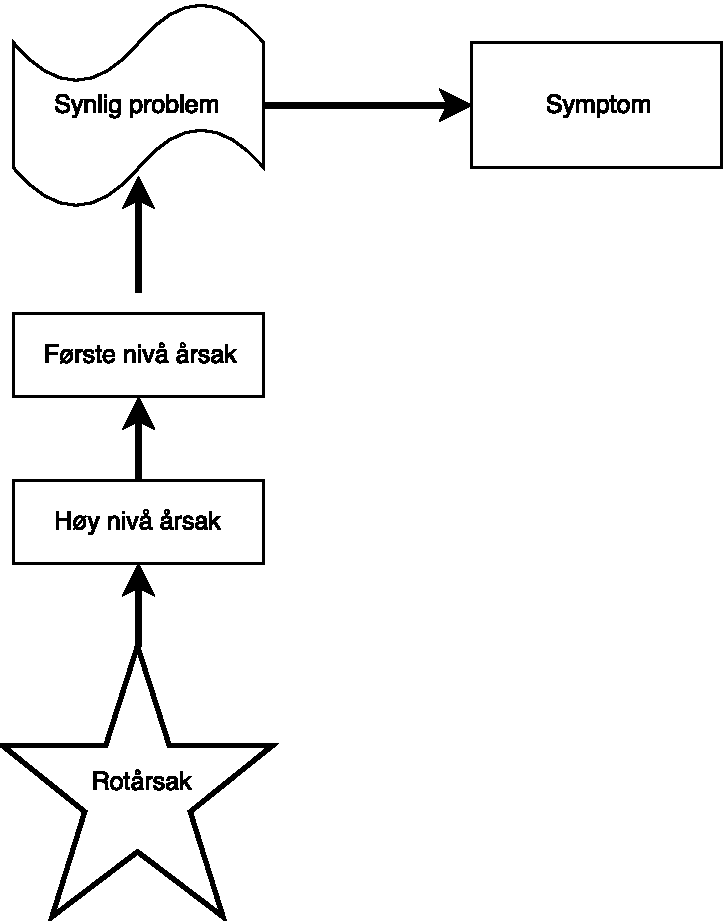
\includegraphics[scale=0.6]{main/bilder/nivaa.pdf}
    \caption[Nivåer av årsaker]{De forskjellige nivåer til problemet}
    \label{fig:nivaa}
\end{figure}

Vi ser fra figuren at rotårsaken er det som setter i gang årsak-virkningskjeden som leder til problemet. 

\subsection{Root Cause Analysis: Simplified tools and techniques}
Denne boken fra 2006 gir en generell beskrivelse av verktøyene og fremgangsmåten til rotårsaksanalyse. 

\subsection{Tidligere arbeid innen informasjonssikkerhet}
I 2016 ga NTNU en bacheloroppgave som innebar bruk av rotårsaksanalyse på tre forskjellige caser \cite{RCARapport}. Oppgaven viste at rotårsakanalyse fungerer i informasjonsikkerhetssammenheng. Vår oppgave skal jobbe videre med å se på hvordan rotårsaksanalyse fungerer i informasjonsikkerhet. OBS: TIL UTBEDRING!

\subsection{Rotårsaksanalyse sammenlignet med risikoanalyse}
En risikoanalyse ser på sannsynlighet for at en trussel kan skje og mulige konsekvenser av dette. Risikoen regnes ut fra sannsynlighet og konsekvens, samt eksisterende kontroller. I risikoanalysen vil dataene brukes til å finne mulige preventive og reaktive tiltak som kan føre riskoen ned på et akseptabelt nivå. Rotårsaksanalyse vil på sin side gjøre en systematisk gjenomgang for å finne de underliggende årsakene til feil eller svikt. En rotårsaksanalyse gjøres etter et problem har oppstått, i motsetning til riskoanalyse som gjøres for å behandle fremtidige situasjoner. 